% !BIB program = bibtex

\documentclass[12pt]{article}

% Font
% \usepackage{fontspec} % need for minion pro
% \usepackage{xunicode}
% \setmainfont[Mapping=tex-text]{Minion Pro} % font
% \setmonofont[Mapping=tex-text,Scale=MatchLowercase,BoldFont={Consolas Bold}]{Consolas} % font

% Non xelatex font options -- bitstream charter
\usepackage[charter,cal=cmcal]{mathdesign}

% Margins
\usepackage[margin = 1in]{geometry}

% Math
\usepackage{amsmath, amsfonts,mathtools}

% Links
\usepackage[colorlinks=true, urlcolor={black}, citecolor={black}, linkcolor={black}]{hyperref}

% Images
\usepackage{graphicx}

% Bold Math Symbols
\usepackage{bm}

% Spacing
\usepackage{setspace}
\doublespacing

% Margin
\usepackage[margin = 1in]{geometry}

% Images -- tikzDevice
\usepackage{tikz}
\usepackage[skip = 0pt]{caption}

% Bibliography
\usepackage[round]{natbib}

\newcommand{\red}{\textcolor{red}}
\newcommand{\blue}{\textcolor{blue}}

\begin{document}
\title{\Large{The Economic Barriers to Arms Races}}
\author{
    Daniel Kent\footnote{\texttt{kent.249@osu.edu}}
    }
\date{\today}
\maketitle


\singlespacing

\begin{abstract} 

\noindent How do states limit the severity of arms races? The security dilemma -- the means by which a state makes itself more secure leave others less secure -- is given pride of place in international relations theory. Beyond the outbreak of war, the economic costs of security dilemma-induced military competitions are generally understood to be mutually undesirable by all sides. 
However, if one compares this rich theoretical tradition to empirical data, then a puzzle emerges. Theory suggests that intense military competition and arms races should be prevalent across time and space. 
Yet in reality most states spend relatively little of their available capital on the military and arms races are the exception, not the norm. 
%Moreover, a closer look at historic arms races and enduring rivalries demonstrates that even in the most-likely candidates for genuine arms races, relationships tend to be asymmetric. Relative capabilities do not reflect a spiral, where each side repeatedly out-arms the other. Rather, in most enduring rivalries one state consistently lags behind another in military size. 
Considering this empirical reality, I argue that arms races are rare not because of a state's ability to signal benign intentions or the possession of defensively-dominant technology. Arms races are rare because very few states can afford them. Most states simply cannot bear the economic costs of military parity or gaining a military advantage over their most powerful neighbors. \emph{In general, the only way to win is not to play.} 
I demonstrate this argument through a computational model of military spending. In the model agents vary in their economic capacity and have to balance competing economic and security pressures when deciding whether to grow their military. When agents are faced with a guns-butter tradeoff and possess realistic economic traits, the model produces simulated results that closely mirror real-world trends in military spending. I conclude with remarks about next steps and a brief discussion of the model's implications for related literatures, such as the emergence of hierarchies and alliance coalitions. % The loss of autonomy associated with hierarchies and alliances is the cost, but the benefits increase the more a state is unable to externally meet its environmental needs. %The model implies two novel pathways for states seeking to end ongoing military competitions. (1) If one state's economy is substantially bigger than another's, then flooding the market and arming up exponentially can price the other state(s) out of military competition. (2) If pathways to increasing another state's domestic economic costs are available, then these can decrease their ability to continue arming as well.

\end{abstract}

\newpage
\doublespacing
\section{Introduction}

How do states limit the severity of arms races? Since \citeauthor{jervis1978}' (\citeyear{jervis1978}) seminal article, the security dilemma has been given pride-of-place in international relations theory. The core idea is both concise and intuitive: the means by which a state increases its security make other states less secure. When states arm, even for defensive purposes, other states are threatened because those arms could be used offensively; one state's military growth leads other states to arm in response. A spiral of repeated arming and insecurity follows, potentially leading to war. 

Beyond its link to the outbreak of war, the security dilemma is tragic because of the economic costs incurred from reciprocal arming \citep{fearon2018} and the erosion of trust it induces between states. \citep{kydd2007trust} Economically, when entrapped in the security dilemma all states are spending more on their militaries than they would be otherwise. Even worse, these states are argued to be no more secure than they were in the first place because all sides' relative capabilities have not budged. Inversely, if states in an arms race could agree to stop arming and instead reduce spending equally on all sides, then relative arms levels would remain unchanged and each state would free up capital for non-military means. The inability of states to do so has puzzled scholars and produced lengthy debates over the general ``costs of anarchy” \citeauthor{fearon2018} (\citeyear{fearon2018}) – or simply how much states can cooperate over arms level when there is no world government to enforce disputes.

In this paper I present a puzzling gap between theory and reality. While most theoretical arguments about the ways in which states can escape or mitigate the security dilemma have been brought under reasonable question, actual trends are far less troubling. Arms races are rare and states tend to spend a small amount on their military relative to their gdp and overall government expenditures. Theory alone would suggest that states should be maintaining far larger militaries then they do and that arms races should be deeply prevalent. Why is this not the case? I argue that arms races and the security dilemma are primarily mitigated by economic pressures, not credible signals of intentions \citep{schultz2001looking,snyder2011cost} or defensive-dominant technologies. \citep{van1998offense} Compared to their security environment, most states lack the economic capacity to even maintain military parity with their potential adversaries.

To demonstrate this argument, I compare the results of a computational model to real-world trends in military spending and economic activity. In the model agents represents states and start with realistic economic conditions. At each turn agents decide how much to spend on their military based upon their security environment and available economic resources. Throughout, agents face a guns-butter tradeoff where expanding the military draws upon a finite pool of available resources. After walking through the model I compare its simulated results to observational data.


\section{Literature}\footnote{This is a short review. The final paper will have a much longer discussion of existing work.}
The literature on the spiral model has long hypothesized two variables which serve to limit the severity of arms races: the offense-defense balance and how clearly offensive intentions can be distinguished from defensive intentions. The logic is fairly straightforward. The more military technology favors defense, then the less one state arming threatens the security of another. On the other hand, if technology is offense-dominant, then arming inherently is more threatening to the security of others. Moreover, if states can credibly signal that the purpose of their arming is strictly defensive, then other states may avoid arming in return.

However, both mechanisms have come under strong criticisms. As \citet{biddle2001} and \citet{glaser1998} have demonstrated, the offense-defense balance is an extremely unclear concept in practice, and most defensive weapons can be easily converted into useful offensive purposes. Moreover, intentions might be defensive at one moment, but they can easily change. \citep{copeland2000} Uncertainty about \textit{future} intentions means that it may be rational to arm in return, even if intentions are defensive at the present. Strategic environments can shift, as can domestic political preferences. Furthermore, it is unclear if states can even credibly signal defensive intentions, because of the incentives to misrepresent capabilities. \citep{fearon1995}

\section{Looking at the data}

This discussion presents a puzzling juncture. The logic of the security dilemma is persuasive. It makes sense that even defense-oriented security measures often make other states less secure. One can see how states would arm intensely in response to other states arming, and it is unclear how to easily escape these spirals of insecurity and mistrust. And there certainly are anecdotal cases of tensions around military capabilities which could be used for offensive purposes. In figure 1 we see the two cases that have driven much of the arms-race literature: European powers around WWI and the US-USSR arms race during the Cold War. Unsurprisingly, Each country's military spending maps tightly to others.

\vspace{1em}

\begin{figure}[!h]
\begin{center}\resizebox{0.95\linewidth}{!}{% Resize table to fit within \linewidth
% horizontally
% Created by tikzDevice version 0.10.1 on 2018-03-04 15:38:57
% !TEX encoding = UTF-8 Unicode
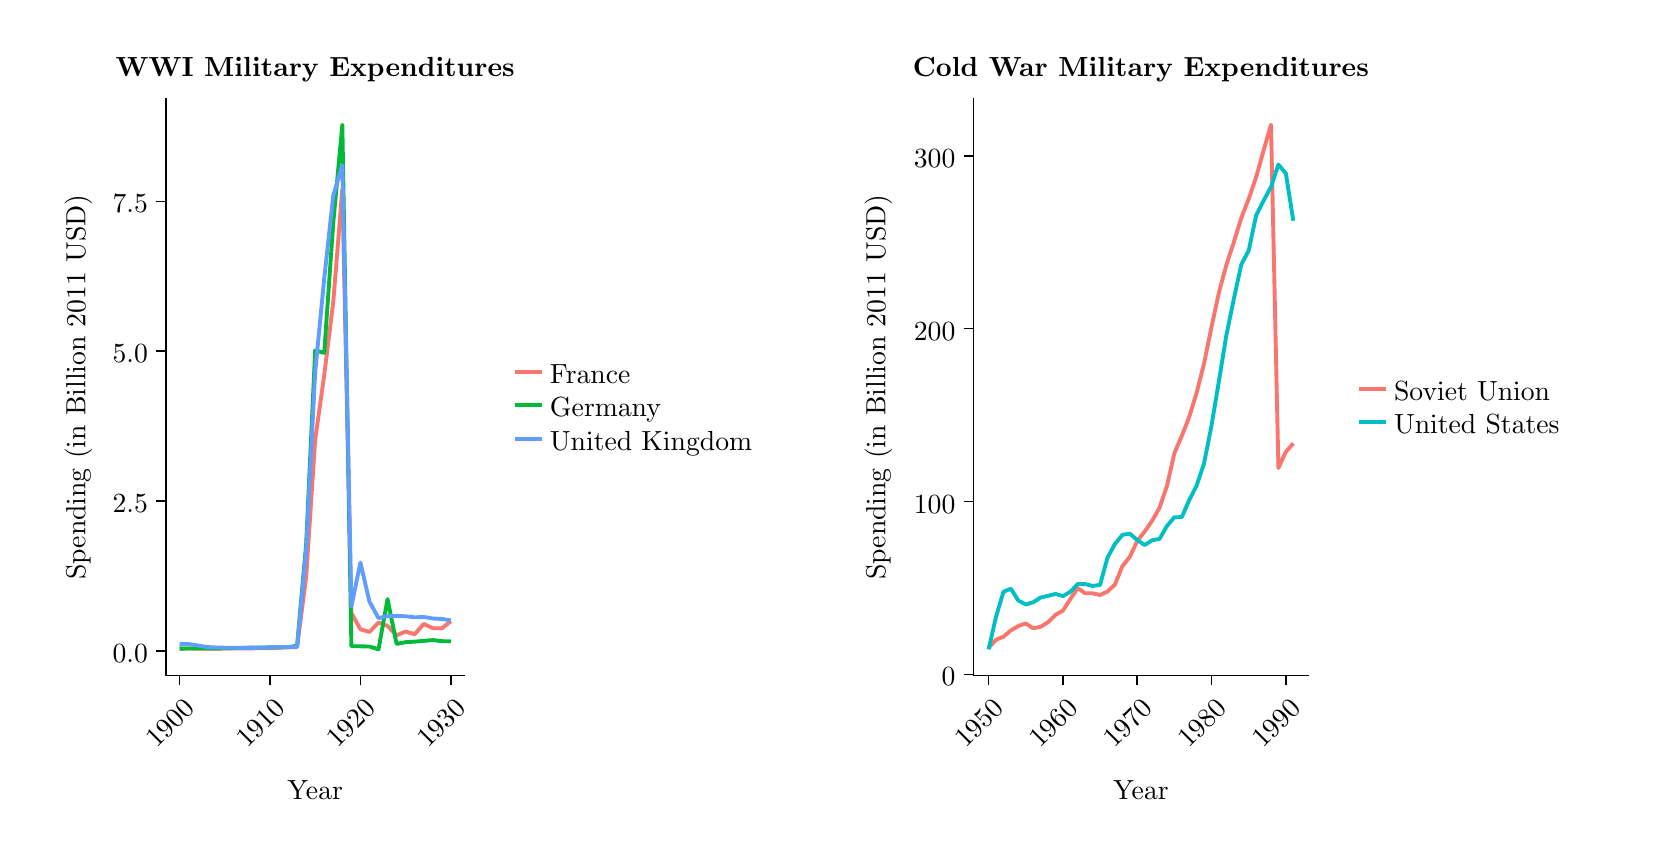
\begin{tikzpicture}[x=1pt,y=1pt]
\definecolor{fillColor}{RGB}{255,255,255}
\path[use as bounding box,fill=fillColor,fill opacity=0.00] (0,0) rectangle (578.16,289.08);
\begin{scope}
\path[clip] ( 49.97, 54.95) rectangle (157.82,263.47);
\definecolor{drawColor}{RGB}{248,118,109}

\path[draw=drawColor,line width= 1.4pt,line join=round] ( 54.87, 64.71) --
	( 58.14, 64.74) --
	( 61.41, 64.70) --
	( 64.68, 64.68) --
	( 67.94, 64.67) --
	( 71.21, 64.74) --
	( 74.48, 64.82) --
	( 77.75, 64.78) --
	( 81.02, 64.80) --
	( 84.29, 64.85) --
	( 87.55, 64.90) --
	( 90.82, 65.03) --
	( 94.09, 65.16) --
	( 97.36, 65.27) --
	(100.63, 90.58) --
	(103.89,140.19) --
	(107.16,163.56) --
	(110.43,190.01) --
	(113.70,230.80) --
	(116.97, 77.58) --
	(120.24, 71.67) --
	(123.50, 70.73) --
	(126.77, 74.14) --
	(130.04, 72.89) --
	(133.31, 69.50) --
	(136.58, 70.86) --
	(139.85, 69.92) --
	(143.11, 73.62) --
	(146.38, 72.09) --
	(149.65, 72.02) --
	(152.92, 74.63);
\definecolor{drawColor}{RGB}{0,186,56}

\path[draw=drawColor,line width= 1.4pt,line join=round] ( 54.87, 64.69) --
	( 58.14, 64.74) --
	( 61.41, 64.75) --
	( 64.68, 64.74) --
	( 67.94, 64.75) --
	( 71.21, 64.83) --
	( 74.48, 64.88) --
	( 77.75, 64.95) --
	( 81.02, 65.08) --
	( 84.29, 65.10) --
	( 87.55, 65.14) --
	( 90.82, 65.16) --
	( 94.09, 65.21) --
	( 97.36, 65.74) --
	(100.63,102.49) --
	(103.89,172.44) --
	(107.16,171.57) --
	(110.43,218.71) --
	(113.70,254.00) --
	(116.97, 65.56) --
	(120.24, 65.54) --
	(123.50, 65.45) --
	(126.77, 64.43) --
	(130.04, 82.59) --
	(133.31, 66.40) --
	(136.58, 67.03) --
	(139.85, 67.22) --
	(143.11, 67.49) --
	(146.38, 67.79) --
	(149.65, 67.39) --
	(152.92, 67.35);
\definecolor{drawColor}{RGB}{97,156,255}

\path[draw=drawColor,line width= 1.4pt,line join=round] ( 54.87, 66.42) --
	( 58.14, 66.36) --
	( 61.41, 65.85) --
	( 64.68, 65.27) --
	( 67.94, 65.12) --
	( 71.21, 65.03) --
	( 74.48, 65.00) --
	( 77.75, 64.98) --
	( 81.02, 64.95) --
	( 84.29, 65.05) --
	( 87.55, 65.16) --
	( 90.82, 65.24) --
	( 94.09, 65.30) --
	( 97.36, 65.29) --
	(100.63,100.19) --
	(103.89,164.59) --
	(107.16,198.42) --
	(110.43,228.47) --
	(113.70,239.38) --
	(116.97, 79.97) --
	(120.24, 95.79) --
	(123.50, 81.69) --
	(126.77, 75.72) --
	(130.04, 76.48) --
	(133.31, 76.48) --
	(136.58, 76.40) --
	(139.85, 76.02) --
	(143.11, 76.13) --
	(146.38, 75.59) --
	(149.65, 75.41) --
	(152.92, 74.92);
\end{scope}
\begin{scope}
\path[clip] (  0.00,  0.00) rectangle (578.16,289.08);
\definecolor{drawColor}{RGB}{0,0,0}

\path[draw=drawColor,line width= 0.6pt,line join=round,line cap=rect] ( 49.97, 54.95) --
	( 49.97,263.47);
\end{scope}
\begin{scope}
\path[clip] (  0.00,  0.00) rectangle (578.16,289.08);
\definecolor{drawColor}{RGB}{0,0,0}

\node[text=drawColor,anchor=base east,inner sep=0pt, outer sep=0pt, scale=  1.0000] at ( 43.47, 59.70) {0.0};

\node[text=drawColor,anchor=base east,inner sep=0pt, outer sep=0pt, scale=  1.0000] at ( 43.47,113.85) {2.5};

\node[text=drawColor,anchor=base east,inner sep=0pt, outer sep=0pt, scale=  1.0000] at ( 43.47,168.00) {5.0};

\node[text=drawColor,anchor=base east,inner sep=0pt, outer sep=0pt, scale=  1.0000] at ( 43.47,222.16) {7.5};
\end{scope}
\begin{scope}
\path[clip] (  0.00,  0.00) rectangle (578.16,289.08);
\definecolor{drawColor}{RGB}{0,0,0}

\path[draw=drawColor,line width= 0.6pt,line join=round] ( 46.47, 63.83) --
	( 49.97, 63.83);

\path[draw=drawColor,line width= 0.6pt,line join=round] ( 46.47,117.98) --
	( 49.97,117.98);

\path[draw=drawColor,line width= 0.6pt,line join=round] ( 46.47,172.14) --
	( 49.97,172.14);

\path[draw=drawColor,line width= 0.6pt,line join=round] ( 46.47,226.29) --
	( 49.97,226.29);
\end{scope}
\begin{scope}
\path[clip] (  0.00,  0.00) rectangle (578.16,289.08);
\definecolor{drawColor}{RGB}{0,0,0}

\path[draw=drawColor,line width= 0.6pt,line join=round,line cap=rect] ( 49.97, 54.95) --
	(157.82, 54.95);
\end{scope}
\begin{scope}
\path[clip] (  0.00,  0.00) rectangle (578.16,289.08);
\definecolor{drawColor}{RGB}{0,0,0}

\path[draw=drawColor,line width= 0.6pt,line join=round] ( 54.87, 51.45) --
	( 54.87, 54.95);

\path[draw=drawColor,line width= 0.6pt,line join=round] ( 87.55, 51.45) --
	( 87.55, 54.95);

\path[draw=drawColor,line width= 0.6pt,line join=round] (120.24, 51.45) --
	(120.24, 54.95);

\path[draw=drawColor,line width= 0.6pt,line join=round] (152.92, 51.45) --
	(152.92, 54.95);
\end{scope}
\begin{scope}
\path[clip] (  0.00,  0.00) rectangle (578.16,289.08);
\definecolor{drawColor}{RGB}{0,0,0}

\node[text=drawColor,rotate= 45.00,anchor=base east,inner sep=0pt, outer sep=0pt, scale=  1.0000] at ( 60.72, 42.61) {1900};

\node[text=drawColor,rotate= 45.00,anchor=base east,inner sep=0pt, outer sep=0pt, scale=  1.0000] at ( 93.40, 42.61) {1910};

\node[text=drawColor,rotate= 45.00,anchor=base east,inner sep=0pt, outer sep=0pt, scale=  1.0000] at (126.08, 42.61) {1920};

\node[text=drawColor,rotate= 45.00,anchor=base east,inner sep=0pt, outer sep=0pt, scale=  1.0000] at (158.76, 42.61) {1930};
\end{scope}
\begin{scope}
\path[clip] (  0.00,  0.00) rectangle (578.16,289.08);
\definecolor{drawColor}{RGB}{0,0,0}

\node[text=drawColor,anchor=base,inner sep=0pt, outer sep=0pt, scale=  1.0000000] at (103.89, 10.00) {Year};
\end{scope}
\begin{scope}
\path[clip] (  0.00,  0.00) rectangle (578.16,289.08);
\definecolor{drawColor}{RGB}{0,0,0}

\node[text=drawColor,rotate= 90.00,anchor=base,inner sep=0pt, outer sep=0pt, scale=  1.0000000] at ( 20.89,159.21) {Spending (in Billion 2011 USD)};
\end{scope}
\begin{scope}
\path[clip] (  0.00,  0.00) rectangle (578.16,289.08);
\definecolor{drawColor}{RGB}{248,118,109}

\path[draw=drawColor,line width= 1.4pt,line join=round] (176.10,164.63) -- (185.73,164.63);
\end{scope}
\begin{scope}
\path[clip] (  0.00,  0.00) rectangle (578.16,289.08);
\definecolor{drawColor}{RGB}{0,186,56}

\path[draw=drawColor,line width= 1.4pt,line join=round] (176.10,152.58) -- (185.73,152.58);
\end{scope}
\begin{scope}
\path[clip] (  0.00,  0.00) rectangle (578.16,289.08);
\definecolor{drawColor}{RGB}{97,156,255}

\path[draw=drawColor,line width= 1.4pt,line join=round] (176.10,140.54) -- (185.73,140.54);
\end{scope}
\begin{scope}
\path[clip] (  0.00,  0.00) rectangle (578.16,289.08);
\definecolor{drawColor}{RGB}{0,0,0}

\node[text=drawColor,anchor=base west,inner sep=0pt, outer sep=0pt, scale=  1.0000] at (188.74,160.50) {France};
\end{scope}
\begin{scope}
\path[clip] (  0.00,  0.00) rectangle (578.16,289.08);
\definecolor{drawColor}{RGB}{0,0,0}

\node[text=drawColor,anchor=base west,inner sep=0pt, outer sep=0pt, scale=  1.0000] at (188.74,148.45) {Germany};
\end{scope}
\begin{scope}
\path[clip] (  0.00,  0.00) rectangle (578.16,289.08);
\definecolor{drawColor}{RGB}{0,0,0}

\node[text=drawColor,anchor=base west,inner sep=0pt, outer sep=0pt, scale=  1.0000] at (188.74,136.41) {United Kingdom};
\end{scope}
\begin{scope}
\path[clip] (  0.00,  0.00) rectangle (578.16,289.08);
\definecolor{drawColor}{RGB}{0,0,0}

\node[text=drawColor,anchor=base,inner sep=0pt, outer sep=0pt, scale=  1.0000000] at (103.89,271.45) {\bfseries WWI Military Expenditures};
\end{scope}
\begin{scope}
\path[clip] (341.71, 54.95) rectangle (462.83,263.47);
\definecolor{drawColor}{RGB}{248,118,109}

\path[draw=drawColor,line width= 1.4pt,line join=round] (347.22, 65.02) --
	(347.22, 65.02) --
	(349.91, 67.91) --
	(349.91, 67.91) --
	(352.59, 69.02) --
	(352.59, 69.02) --
	(355.28, 71.28) --
	(355.28, 71.28) --
	(357.96, 72.87) --
	(357.96, 72.87) --
	(360.65, 73.79) --
	(360.65, 73.79) --
	(363.33, 72.05) --
	(363.33, 72.05) --
	(366.02, 72.59) --
	(366.02, 72.59) --
	(368.70, 74.23) --
	(368.70, 74.23) --
	(371.39, 76.89) --
	(371.39, 76.89) --
	(374.08, 78.43) --
	(374.08, 78.43) --
	(376.76, 82.62) --
	(376.76, 82.62) --
	(379.45, 86.56) --
	(379.45, 86.56) --
	(382.13, 84.70) --
	(382.13, 84.70) --
	(384.82, 84.70) --
	(384.82, 84.70) --
	(387.50, 84.08) --
	(387.50, 84.08) --
	(390.19, 85.33) --
	(390.19, 85.33) --
	(392.87, 87.83) --
	(392.87, 87.83) --
	(395.56, 94.46) --
	(395.56, 94.46) --
	(398.24, 97.86) --
	(398.24, 97.86) --
	(400.93,103.58) --
	(400.93,103.58) --
	(403.62,107.01) --
	(403.62,107.01) --
	(406.30,110.89) --
	(406.30,110.89) --
	(408.99,115.58) --
	(408.99,115.58) --
	(411.67,123.45) --
	(411.67,123.45) --
	(414.36,135.32) --
	(414.36,135.32) --
	(417.04,141.57) --
	(417.04,141.57) --
	(419.73,148.45) --
	(419.73,148.45) --
	(422.41,157.19) --
	(422.41,157.19) --
	(425.10,167.82) --
	(425.10,167.82) --
	(427.78,180.94) --
	(427.78,180.94) --
	(430.47,193.44) --
	(430.47,193.44) --
	(433.16,203.44) --
	(433.16,203.44) --
	(435.84,211.56) --
	(435.84,211.56) --
	(438.53,220.31) --
	(438.53,220.31) --
	(441.21,227.19) --
	(441.21,227.19) --
	(443.90,235.06) --
	(443.90,235.06) --
	(446.58,244.68) --
	(446.58,244.68) --
	(449.27,254.00) --
	(449.27,254.00) --
	(451.95,129.97) --
	(451.95,129.97) --
	(454.64,135.82) --
	(454.64,135.82) --
	(457.33,138.88) --
	(457.33,138.88);
\definecolor{drawColor}{RGB}{0,191,196}

\path[draw=drawColor,line width= 1.4pt,line join=round] (347.22, 64.43) --
	(349.91, 76.20) --
	(352.59, 85.23) --
	(355.28, 86.34) --
	(357.96, 82.07) --
	(360.65, 80.65) --
	(363.33, 81.44) --
	(366.02, 83.17) --
	(368.70, 83.77) --
	(371.39, 84.46) --
	(374.08, 83.69) --
	(376.76, 85.21) --
	(379.45, 88.06) --
	(382.13, 88.01) --
	(384.82, 87.34) --
	(387.50, 87.72) --
	(390.19, 97.56) --
	(392.87,102.48) --
	(395.56,105.78) --
	(398.24,106.23) --
	(400.93,103.97) --
	(403.62,102.11) --
	(406.30,103.85) --
	(408.99,104.32) --
	(411.67,109.02) --
	(414.36,112.17) --
	(417.04,112.21) --
	(419.73,118.40) --
	(422.41,123.60) --
	(425.10,131.75) --
	(427.78,145.31) --
	(430.47,161.50) --
	(433.16,178.03) --
	(435.84,191.06) --
	(438.53,203.47) --
	(441.21,208.53) --
	(443.90,221.24) --
	(446.58,226.54) --
	(449.27,231.52) --
	(451.95,239.61) --
	(454.64,236.41) --
	(457.33,219.31);
\end{scope}
\begin{scope}
\path[clip] (  0.00,  0.00) rectangle (578.16,289.08);
\definecolor{drawColor}{RGB}{0,0,0}

\path[draw=drawColor,line width= 0.6pt,line join=round,line cap=rect] (341.71, 54.95) --
	(341.71,263.47);
\end{scope}
\begin{scope}
\path[clip] (  0.00,  0.00) rectangle (578.16,289.08);
\definecolor{drawColor}{RGB}{0,0,0}

\node[text=drawColor,anchor=base east,inner sep=0pt, outer sep=0pt, scale=  1.0000] at (335.22, 51.20) {0};

\node[text=drawColor,anchor=base east,inner sep=0pt, outer sep=0pt, scale=  1.0000] at (335.22,113.69) {100};

\node[text=drawColor,anchor=base east,inner sep=0pt, outer sep=0pt, scale=  1.0000] at (335.22,176.18) {200};

\node[text=drawColor,anchor=base east,inner sep=0pt, outer sep=0pt, scale=  1.0000] at (335.22,238.68) {300};
\end{scope}
\begin{scope}
\path[clip] (  0.00,  0.00) rectangle (578.16,289.08);
\definecolor{drawColor}{RGB}{0,0,0}

\path[draw=drawColor,line width= 0.6pt,line join=round] (338.21, 55.33) --
	(341.71, 55.33);

\path[draw=drawColor,line width= 0.6pt,line join=round] (338.21,117.82) --
	(341.71,117.82);

\path[draw=drawColor,line width= 0.6pt,line join=round] (338.21,180.32) --
	(341.71,180.32);

\path[draw=drawColor,line width= 0.6pt,line join=round] (338.21,242.81) --
	(341.71,242.81);
\end{scope}
\begin{scope}
\path[clip] (  0.00,  0.00) rectangle (578.16,289.08);
\definecolor{drawColor}{RGB}{0,0,0}

\path[draw=drawColor,line width= 0.6pt,line join=round,line cap=rect] (341.71, 54.95) --
	(462.83, 54.95);
\end{scope}
\begin{scope}
\path[clip] (  0.00,  0.00) rectangle (578.16,289.08);
\definecolor{drawColor}{RGB}{0,0,0}

\path[draw=drawColor,line width= 0.6pt,line join=round] (347.22, 51.45) --
	(347.22, 54.95);

\path[draw=drawColor,line width= 0.6pt,line join=round] (374.08, 51.45) --
	(374.08, 54.95);

\path[draw=drawColor,line width= 0.6pt,line join=round] (400.93, 51.45) --
	(400.93, 54.95);

\path[draw=drawColor,line width= 0.6pt,line join=round] (427.78, 51.45) --
	(427.78, 54.95);

\path[draw=drawColor,line width= 0.6pt,line join=round] (454.64, 51.45) --
	(454.64, 54.95);
\end{scope}
\begin{scope}
\path[clip] (  0.00,  0.00) rectangle (578.16,289.08);
\definecolor{drawColor}{RGB}{0,0,0}

\node[text=drawColor,rotate= 45.00,anchor=base east,inner sep=0pt, outer sep=0pt, scale=  1.0000] at (353.06, 42.61) {1950};

\node[text=drawColor,rotate= 45.00,anchor=base east,inner sep=0pt, outer sep=0pt, scale=  1.0000] at (379.92, 42.61) {1960};

\node[text=drawColor,rotate= 45.00,anchor=base east,inner sep=0pt, outer sep=0pt, scale=  1.0000] at (406.77, 42.61) {1970};

\node[text=drawColor,rotate= 45.00,anchor=base east,inner sep=0pt, outer sep=0pt, scale=  1.0000] at (433.63, 42.61) {1980};

\node[text=drawColor,rotate= 45.00,anchor=base east,inner sep=0pt, outer sep=0pt, scale=  1.0000] at (460.48, 42.61) {1990};
\end{scope}
\begin{scope}
\path[clip] (  0.00,  0.00) rectangle (578.16,289.08);
\definecolor{drawColor}{RGB}{0,0,0}

\node[text=drawColor,anchor=base,inner sep=0pt, outer sep=0pt, scale=  1.0000000] at (402.27, 10.00) {Year};
\end{scope}
\begin{scope}
\path[clip] (  0.00,  0.00) rectangle (578.16,289.08);
\definecolor{drawColor}{RGB}{0,0,0}

\node[text=drawColor,rotate= 90.00,anchor=base,inner sep=0pt, outer sep=0pt, scale=  1.0000000] at (309.97,159.21) {Spending (in Billion 2011 USD)};
\end{scope}
\begin{scope}
\path[clip] (  0.00,  0.00) rectangle (578.16,289.08);
\definecolor{drawColor}{RGB}{248,118,109}

\path[draw=drawColor,line width= 1.4pt,line join=round] (481.11,158.61) -- (490.74,158.61);
\end{scope}
\begin{scope}
\path[clip] (  0.00,  0.00) rectangle (578.16,289.08);
\definecolor{drawColor}{RGB}{0,191,196}

\path[draw=drawColor,line width= 1.4pt,line join=round] (481.11,146.56) -- (490.74,146.56);
\end{scope}
\begin{scope}
\path[clip] (  0.00,  0.00) rectangle (578.16,289.08);
\definecolor{drawColor}{RGB}{0,0,0}

\node[text=drawColor,anchor=base west,inner sep=0pt, outer sep=0pt, scale=  1.0000] at (493.75,154.47) {Soviet Union};
\end{scope}
\begin{scope}
\path[clip] (  0.00,  0.00) rectangle (578.16,289.08);
\definecolor{drawColor}{RGB}{0,0,0}

\node[text=drawColor,anchor=base west,inner sep=0pt, outer sep=0pt, scale=  1.0000] at (493.75,142.43) {United States};
\end{scope}
\begin{scope}
\path[clip] (  0.00,  0.00) rectangle (578.16,289.08);
\definecolor{drawColor}{RGB}{0,0,0}

\node[text=drawColor,anchor=base,inner sep=0pt, outer sep=0pt, scale=  1.0000000] at (402.27,271.45) {\bfseries Cold War Military Expenditures};
\end{scope}
\end{tikzpicture}

}
\caption{Arms races during World War I and the Cold War. For each figure the y-axis corresponds to military spending.}
\end{center}
\end{figure}


But when we look at military spending across two prominent enduring rivalries -- where underlying disputes provide good reason for each state to seek a military advantage -- we see that in both cases one state lags substantially behind the other. This dynamic is displayed in figure 2. Certainly there is a correlation and both states are considering the other when investing in military capabilities. But in both cases we do not see the expected reciprocal spiral of one state gaining a military advantage and another state arming to regain an advantage, as arms races tend to be portrayed. Rather, the relationship is asymmetric, with one state trying to keep up with the other out of fear of subservience and attack. In this sense, it is not clear that the relationship is characterized by an arms race, or a smaller state doing its best to keep up with the larger state. India's economic capacity is far greater than Pakistan's. Saudi Arabia can afford a larger military than Iran due to oil exports. Although simple, to the best of my knowledge this point has not been made: in all but the most extreme scenarios the security dilemma is somewhat irrelevant because one or more states cannot afford spirals of mistrust and reciprocal arming.

\begin{figure}[!h]
    \begin{center}
        \resizebox{0.95\linewidth}{!}{%
            % Created by tikzDevice version 0.10.1 on 2018-03-04 17:10:26
% !TEX encoding = UTF-8 Unicode
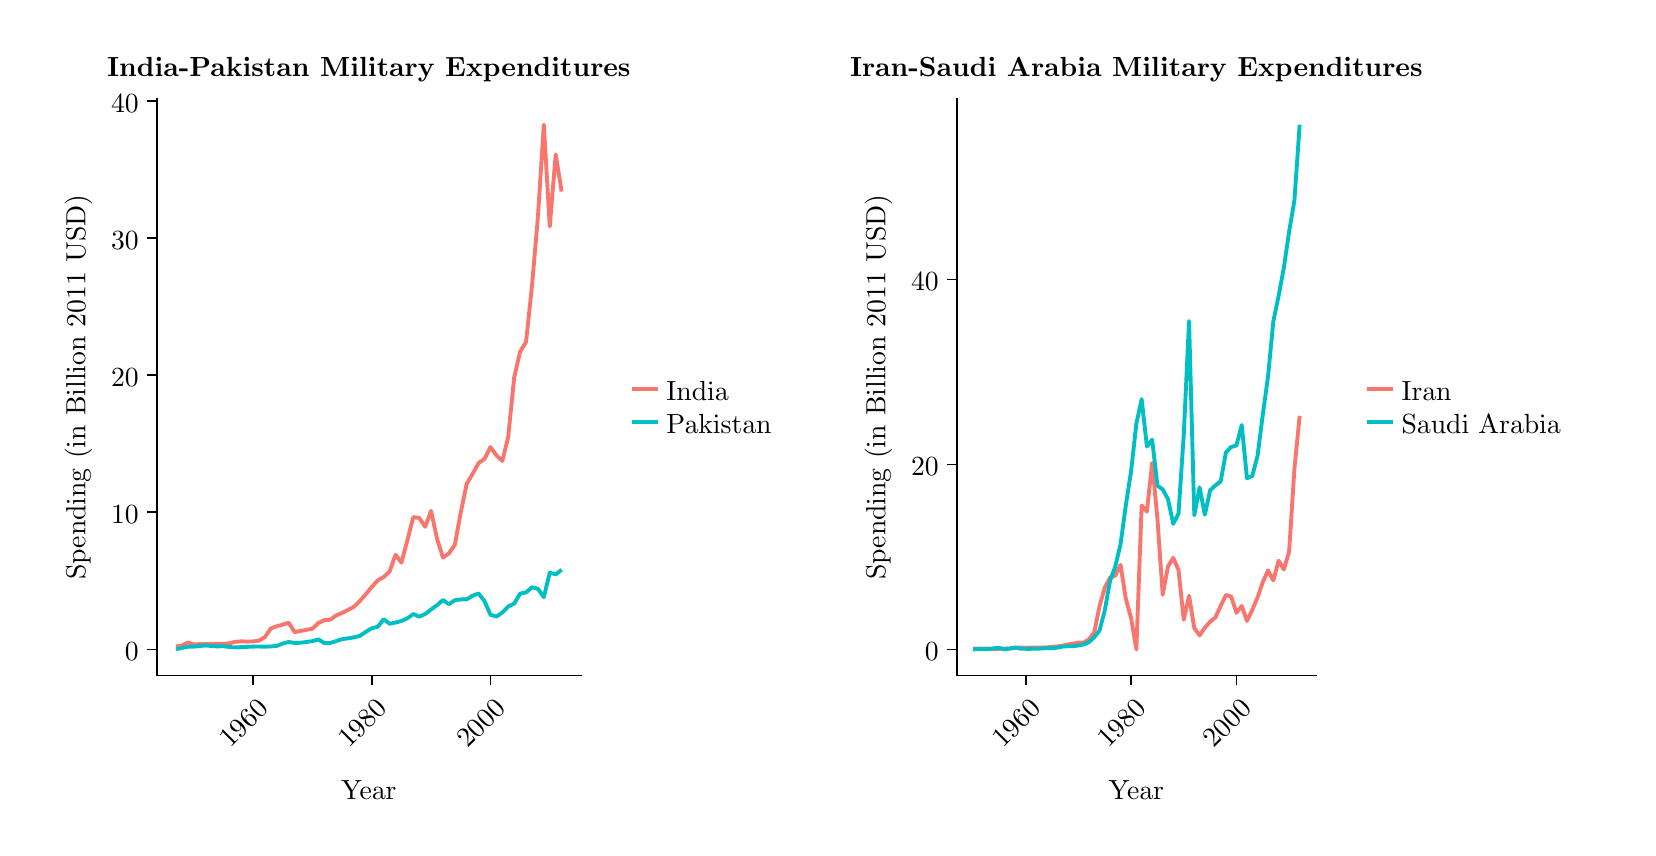
\begin{tikzpicture}[x=1pt,y=1pt]
\definecolor{fillColor}{RGB}{255,255,255}
\path[use as bounding box,fill=fillColor,fill opacity=0.00] (0,0) rectangle (578.16,289.08);
\begin{scope}
\path[clip] ( 46.64, 54.95) rectangle (199.91,263.47);
\definecolor{drawColor}{RGB}{248,118,109}

\path[draw=drawColor,line width= 1.4pt,line join=round] ( 53.60, 65.51) --
	( 55.75, 65.79) --
	( 57.89, 66.92) --
	( 60.03, 66.24) --
	( 62.18, 66.33) --
	( 64.32, 66.36) --
	( 66.47, 66.43) --
	( 68.61, 66.47) --
	( 70.75, 66.42) --
	( 72.90, 66.62) --
	( 75.04, 67.18) --
	( 77.18, 67.33) --
	( 79.33, 67.23) --
	( 81.47, 67.30) --
	( 83.62, 67.59) --
	( 85.76, 68.94) --
	( 87.90, 72.01) --
	( 90.05, 72.80) --
	( 92.19, 73.36) --
	( 94.33, 74.05) --
	( 96.48, 70.66) --
	( 98.62, 71.10) --
	(100.76, 71.48) --
	(102.91, 71.90) --
	(105.05, 73.96) --
	(107.20, 75.00) --
	(109.34, 75.14) --
	(111.48, 76.68) --
	(113.63, 77.60) --
	(115.77, 78.69) --
	(117.91, 79.83) --
	(120.06, 81.94) --
	(122.20, 84.36) --
	(124.35, 87.02) --
	(126.49, 89.30) --
	(128.63, 90.57) --
	(130.78, 92.57) --
	(132.92, 98.64) --
	(135.06, 95.78) --
	(137.21,103.90) --
	(139.35,112.22) --
	(141.49,111.92) --
	(143.64,108.70) --
	(145.78,114.45) --
	(147.93,104.39) --
	(150.07, 97.61) --
	(152.21, 99.10) --
	(154.36,102.26) --
	(156.50,113.91) --
	(158.64,124.25) --
	(160.79,127.84) --
	(162.93,131.75) --
	(165.08,133.24) --
	(167.22,137.55) --
	(169.36,134.59) --
	(171.51,132.52) --
	(173.65,141.23) --
	(175.79,162.59) --
	(177.94,172.02) --
	(180.08,175.50) --
	(182.23,195.73) --
	(184.37,220.63) --
	(186.51,254.00) --
	(188.66,217.28) --
	(190.80,243.28) --
	(192.94,229.86);
\definecolor{drawColor}{RGB}{0,191,196}

\path[draw=drawColor,line width= 1.4pt,line join=round] ( 53.60, 64.43) --
	( 55.75, 64.96) --
	( 57.89, 65.36) --
	( 60.03, 65.42) --
	( 62.18, 65.64) --
	( 64.32, 65.83) --
	( 66.47, 65.65) --
	( 68.61, 65.48) --
	( 70.75, 65.60) --
	( 72.90, 65.25) --
	( 75.04, 65.17) --
	( 77.18, 65.23) --
	( 79.33, 65.34) --
	( 81.47, 65.44) --
	( 83.62, 65.45) --
	( 85.76, 65.40) --
	( 87.90, 65.49) --
	( 90.05, 65.68) --
	( 92.19, 66.55) --
	( 94.33, 67.10) --
	( 96.48, 66.74) --
	( 98.62, 66.82) --
	(100.76, 67.10) --
	(102.91, 67.41) --
	(105.05, 68.03) --
	(107.20, 66.69) --
	(109.34, 66.76) --
	(111.48, 67.40) --
	(113.63, 68.14) --
	(115.77, 68.41) --
	(117.91, 68.78) --
	(120.06, 69.32) --
	(122.20, 70.76) --
	(124.35, 72.07) --
	(126.49, 72.59) --
	(128.63, 75.33) --
	(130.78, 73.70) --
	(132.92, 74.12) --
	(135.06, 74.67) --
	(137.21, 75.67) --
	(139.35, 77.21) --
	(141.49, 76.22) --
	(143.64, 77.21) --
	(145.78, 78.84) --
	(147.93, 80.42) --
	(150.07, 82.26) --
	(152.21, 80.77) --
	(154.36, 82.18) --
	(156.50, 82.47) --
	(158.64, 82.51) --
	(160.79, 83.82) --
	(162.93, 84.62) --
	(165.08, 81.88) --
	(167.22, 76.92) --
	(169.36, 76.29) --
	(171.51, 77.74) --
	(173.65, 79.92) --
	(175.79, 80.96) --
	(177.94, 84.57) --
	(180.08, 85.01) --
	(182.23, 86.86) --
	(184.37, 86.33) --
	(186.51, 83.30) --
	(188.66, 92.16) --
	(190.80, 91.51) --
	(192.94, 93.22);
\end{scope}
\begin{scope}
\path[clip] (  0.00,  0.00) rectangle (578.16,289.08);
\definecolor{drawColor}{RGB}{0,0,0}

\path[draw=drawColor,line width= 0.6pt,line join=round,line cap=rect] ( 46.64, 54.95) --
	( 46.64,263.47);
\end{scope}
\begin{scope}
\path[clip] (  0.00,  0.00) rectangle (578.16,289.08);
\definecolor{drawColor}{RGB}{0,0,0}

\node[text=drawColor,anchor=base east,inner sep=0pt, outer sep=0pt, scale=  1.0000] at ( 40.14, 60.30) {0};

\node[text=drawColor,anchor=base east,inner sep=0pt, outer sep=0pt, scale=  1.0000] at ( 40.14,109.82) {10};

\node[text=drawColor,anchor=base east,inner sep=0pt, outer sep=0pt, scale=  1.0000] at ( 40.14,159.34) {20};

\node[text=drawColor,anchor=base east,inner sep=0pt, outer sep=0pt, scale=  1.0000] at ( 40.14,208.87) {30};

\node[text=drawColor,anchor=base east,inner sep=0pt, outer sep=0pt, scale=  1.0000] at ( 40.14,258.39) {40};
\end{scope}
\begin{scope}
\path[clip] (  0.00,  0.00) rectangle (578.16,289.08);
\definecolor{drawColor}{RGB}{0,0,0}

\path[draw=drawColor,line width= 0.6pt,line join=round] ( 43.14, 64.43) --
	( 46.64, 64.43);

\path[draw=drawColor,line width= 0.6pt,line join=round] ( 43.14,113.95) --
	( 46.64,113.95);

\path[draw=drawColor,line width= 0.6pt,line join=round] ( 43.14,163.48) --
	( 46.64,163.48);

\path[draw=drawColor,line width= 0.6pt,line join=round] ( 43.14,213.00) --
	( 46.64,213.00);

\path[draw=drawColor,line width= 0.6pt,line join=round] ( 43.14,262.52) --
	( 46.64,262.52);
\end{scope}
\begin{scope}
\path[clip] (  0.00,  0.00) rectangle (578.16,289.08);
\definecolor{drawColor}{RGB}{0,0,0}

\path[draw=drawColor,line width= 0.6pt,line join=round,line cap=rect] ( 46.64, 54.95) --
	(199.91, 54.95);
\end{scope}
\begin{scope}
\path[clip] (  0.00,  0.00) rectangle (578.16,289.08);
\definecolor{drawColor}{RGB}{0,0,0}

\path[draw=drawColor,line width= 0.6pt,line join=round] ( 81.47, 51.45) --
	( 81.47, 54.95);

\path[draw=drawColor,line width= 0.6pt,line join=round] (124.35, 51.45) --
	(124.35, 54.95);

\path[draw=drawColor,line width= 0.6pt,line join=round] (167.22, 51.45) --
	(167.22, 54.95);
\end{scope}
\begin{scope}
\path[clip] (  0.00,  0.00) rectangle (578.16,289.08);
\definecolor{drawColor}{RGB}{0,0,0}

\node[text=drawColor,rotate= 45.00,anchor=base east,inner sep=0pt, outer sep=0pt, scale=  1.0000] at ( 87.32, 42.61) {1960};

\node[text=drawColor,rotate= 45.00,anchor=base east,inner sep=0pt, outer sep=0pt, scale=  1.0000] at (130.19, 42.61) {1980};

\node[text=drawColor,rotate= 45.00,anchor=base east,inner sep=0pt, outer sep=0pt, scale=  1.0000] at (173.06, 42.61) {2000};
\end{scope}
\begin{scope}
\path[clip] (  0.00,  0.00) rectangle (578.16,289.08);
\definecolor{drawColor}{RGB}{0,0,0}

\node[text=drawColor,anchor=base,inner sep=0pt, outer sep=0pt, scale=  1.0000000] at (123.27, 10.00) {Year};
\end{scope}
\begin{scope}
\path[clip] (  0.00,  0.00) rectangle (578.16,289.08);
\definecolor{drawColor}{RGB}{0,0,0}

\node[text=drawColor,rotate= 90.00,anchor=base,inner sep=0pt, outer sep=0pt, scale=  1.0000000] at ( 20.89,159.21) {Spending (in Billion 2011 USD)};
\end{scope}
\begin{scope}
\path[clip] (  0.00,  0.00) rectangle (578.16,289.08);
\definecolor{drawColor}{RGB}{248,118,109}

\path[draw=drawColor,line width= 1.4pt,line join=round] (218.19,158.61) -- (227.82,158.61);
\end{scope}
\begin{scope}
\path[clip] (  0.00,  0.00) rectangle (578.16,289.08);
\definecolor{drawColor}{RGB}{0,191,196}

\path[draw=drawColor,line width= 1.4pt,line join=round] (218.19,146.56) -- (227.82,146.56);
\end{scope}
\begin{scope}
\path[clip] (  0.00,  0.00) rectangle (578.16,289.08);
\definecolor{drawColor}{RGB}{0,0,0}

\node[text=drawColor,anchor=base west,inner sep=0pt, outer sep=0pt, scale=  1.0000] at (230.83,154.47) {India};
\end{scope}
\begin{scope}
\path[clip] (  0.00,  0.00) rectangle (578.16,289.08);
\definecolor{drawColor}{RGB}{0,0,0}

\node[text=drawColor,anchor=base west,inner sep=0pt, outer sep=0pt, scale=  1.0000] at (230.83,142.43) {Pakistan};
\end{scope}
\begin{scope}
\path[clip] (  0.00,  0.00) rectangle (578.16,289.08);
\definecolor{drawColor}{RGB}{0,0,0}

\node[text=drawColor,anchor=base,inner sep=0pt, outer sep=0pt, scale=  1.0000000] at (123.27,271.45) {\bfseries India-Pakistan Military Expenditures};
\end{scope}
\begin{scope}
\path[clip] (335.72, 54.95) rectangle (465.53,263.47);
\definecolor{drawColor}{RGB}{248,118,109}

\path[draw=drawColor,line width= 1.4pt,line join=round] (341.62, 64.68) --
	(343.52, 64.68) --
	(345.42, 64.69) --
	(347.33, 64.69) --
	(349.23, 64.56) --
	(351.13, 64.62) --
	(353.04, 64.70) --
	(354.94, 64.77) --
	(356.84, 64.98) --
	(358.75, 65.11) --
	(360.65, 65.03) --
	(362.55, 65.05) --
	(364.46, 65.05) --
	(366.36, 65.07) --
	(368.26, 65.16) --
	(370.17, 65.35) --
	(372.07, 65.48) --
	(373.98, 65.80) --
	(375.88, 66.18) --
	(377.78, 66.52) --
	(379.69, 66.89) --
	(381.59, 66.89) --
	(383.49, 68.06) --
	(385.40, 70.49) --
	(387.30, 80.00) --
	(389.20, 86.71) --
	(391.11, 90.32) --
	(393.01, 91.07) --
	(394.91, 94.97) --
	(396.82, 82.69) --
	(398.72, 75.75) --
	(400.62, 64.43) --
	(402.53,116.40) --
	(404.43,114.23) --
	(406.33,131.81) --
	(408.24,111.52) --
	(410.14, 84.15) --
	(412.04, 94.37) --
	(413.95, 97.51) --
	(415.85, 93.17) --
	(417.75, 75.12) --
	(419.66, 83.81) --
	(421.56, 72.12) --
	(423.46, 69.50) --
	(425.37, 72.25) --
	(427.27, 74.45) --
	(429.17, 75.93) --
	(431.08, 80.12) --
	(432.98, 84.08) --
	(434.88, 83.51) --
	(436.79, 77.65) --
	(438.69, 80.13) --
	(440.59, 74.71) --
	(442.50, 78.70) --
	(444.40, 83.16) --
	(446.31, 88.74) --
	(448.21, 92.97) --
	(450.11, 89.33) --
	(452.02, 96.49) --
	(453.92, 93.29) --
	(455.82, 99.73) --
	(457.73,129.63) --
	(459.63,148.81);
\definecolor{drawColor}{RGB}{0,191,196}

\path[draw=drawColor,line width= 1.4pt,line join=round] (341.62, 64.43) --
	(343.52, 64.51) --
	(345.42, 64.49) --
	(347.33, 64.55) --
	(349.23, 64.84) --
	(351.13, 64.94) --
	(353.04, 64.43) --
	(354.94, 64.73) --
	(356.84, 65.11) --
	(358.75, 64.67) --
	(360.65, 64.63) --
	(362.55, 64.63) --
	(364.46, 64.67) --
	(366.36, 64.74) --
	(368.26, 64.84) --
	(370.17, 64.87) --
	(372.07, 65.03) --
	(373.98, 65.44) --
	(375.88, 65.55) --
	(377.78, 65.56) --
	(379.69, 65.85) --
	(381.59, 66.20) --
	(383.49, 67.05) --
	(385.40, 68.79) --
	(387.30, 71.21) --
	(389.20, 78.47) --
	(391.11, 89.20) --
	(393.01, 94.38) --
	(394.91,102.46) --
	(396.82,116.52) --
	(398.72,128.80) --
	(400.62,145.97) --
	(402.53,154.87) --
	(404.43,137.69) --
	(406.33,140.20) --
	(408.24,123.56) --
	(410.14,122.24) --
	(412.04,118.70) --
	(413.95,109.78) --
	(415.85,113.52) --
	(417.75,141.96) --
	(419.66,183.07) --
	(421.56,112.85) --
	(423.46,122.97) --
	(425.37,113.07) --
	(427.27,121.90) --
	(429.17,123.68) --
	(431.08,125.09) --
	(432.98,135.62) --
	(434.88,137.54) --
	(436.79,138.12) --
	(438.69,145.52) --
	(440.59,126.26) --
	(442.50,127.08) --
	(444.40,134.31) --
	(446.31,149.22) --
	(448.21,163.15) --
	(450.11,182.89) --
	(452.02,192.17) --
	(453.92,202.37) --
	(455.82,215.38) --
	(457.73,226.62) --
	(459.63,254.00);
\end{scope}
\begin{scope}
\path[clip] (  0.00,  0.00) rectangle (578.16,289.08);
\definecolor{drawColor}{RGB}{0,0,0}

\path[draw=drawColor,line width= 0.6pt,line join=round,line cap=rect] (335.72, 54.95) --
	(335.72,263.47);
\end{scope}
\begin{scope}
\path[clip] (  0.00,  0.00) rectangle (578.16,289.08);
\definecolor{drawColor}{RGB}{0,0,0}

\node[text=drawColor,anchor=base east,inner sep=0pt, outer sep=0pt, scale=  1.0000] at (329.22, 60.30) {0};

\node[text=drawColor,anchor=base east,inner sep=0pt, outer sep=0pt, scale=  1.0000] at (329.22,127.13) {20};

\node[text=drawColor,anchor=base east,inner sep=0pt, outer sep=0pt, scale=  1.0000] at (329.22,193.97) {40};
\end{scope}
\begin{scope}
\path[clip] (  0.00,  0.00) rectangle (578.16,289.08);
\definecolor{drawColor}{RGB}{0,0,0}

\path[draw=drawColor,line width= 0.6pt,line join=round] (332.22, 64.43) --
	(335.72, 64.43);

\path[draw=drawColor,line width= 0.6pt,line join=round] (332.22,131.27) --
	(335.72,131.27);

\path[draw=drawColor,line width= 0.6pt,line join=round] (332.22,198.11) --
	(335.72,198.11);
\end{scope}
\begin{scope}
\path[clip] (  0.00,  0.00) rectangle (578.16,289.08);
\definecolor{drawColor}{RGB}{0,0,0}

\path[draw=drawColor,line width= 0.6pt,line join=round,line cap=rect] (335.72, 54.95) --
	(465.53, 54.95);
\end{scope}
\begin{scope}
\path[clip] (  0.00,  0.00) rectangle (578.16,289.08);
\definecolor{drawColor}{RGB}{0,0,0}

\path[draw=drawColor,line width= 0.6pt,line join=round] (360.65, 51.45) --
	(360.65, 54.95);

\path[draw=drawColor,line width= 0.6pt,line join=round] (398.72, 51.45) --
	(398.72, 54.95);

\path[draw=drawColor,line width= 0.6pt,line join=round] (436.79, 51.45) --
	(436.79, 54.95);
\end{scope}
\begin{scope}
\path[clip] (  0.00,  0.00) rectangle (578.16,289.08);
\definecolor{drawColor}{RGB}{0,0,0}

\node[text=drawColor,rotate= 45.00,anchor=base east,inner sep=0pt, outer sep=0pt, scale=  1.0000] at (366.50, 42.61) {1960};

\node[text=drawColor,rotate= 45.00,anchor=base east,inner sep=0pt, outer sep=0pt, scale=  1.0000] at (404.56, 42.61) {1980};

\node[text=drawColor,rotate= 45.00,anchor=base east,inner sep=0pt, outer sep=0pt, scale=  1.0000] at (442.63, 42.61) {2000};
\end{scope}
\begin{scope}
\path[clip] (  0.00,  0.00) rectangle (578.16,289.08);
\definecolor{drawColor}{RGB}{0,0,0}

\node[text=drawColor,anchor=base,inner sep=0pt, outer sep=0pt, scale=  1.0000000] at (400.62, 10.00) {Year};
\end{scope}
\begin{scope}
\path[clip] (  0.00,  0.00) rectangle (578.16,289.08);
\definecolor{drawColor}{RGB}{0,0,0}

\node[text=drawColor,rotate= 90.00,anchor=base,inner sep=0pt, outer sep=0pt, scale=  1.0000000] at (309.97,159.21) {Spending (in Billion 2011 USD)};
\end{scope}
\begin{scope}
\path[clip] (  0.00,  0.00) rectangle (578.16,289.08);
\definecolor{drawColor}{RGB}{248,118,109}

\path[draw=drawColor,line width= 1.4pt,line join=round] (483.81,158.61) -- (493.44,158.61);
\end{scope}
\begin{scope}
\path[clip] (  0.00,  0.00) rectangle (578.16,289.08);
\definecolor{drawColor}{RGB}{0,191,196}

\path[draw=drawColor,line width= 1.4pt,line join=round] (483.81,146.56) -- (493.44,146.56);
\end{scope}
\begin{scope}
\path[clip] (  0.00,  0.00) rectangle (578.16,289.08);
\definecolor{drawColor}{RGB}{0,0,0}

\node[text=drawColor,anchor=base west,inner sep=0pt, outer sep=0pt, scale=  1.0000] at (496.45,154.47) {Iran};
\end{scope}
\begin{scope}
\path[clip] (  0.00,  0.00) rectangle (578.16,289.08);
\definecolor{drawColor}{RGB}{0,0,0}

\node[text=drawColor,anchor=base west,inner sep=0pt, outer sep=0pt, scale=  1.0000] at (496.45,142.43) {Saudi Arabia};
\end{scope}
\begin{scope}
\path[clip] (  0.00,  0.00) rectangle (578.16,289.08);
\definecolor{drawColor}{RGB}{0,0,0}

\node[text=drawColor,anchor=base,inner sep=0pt, outer sep=0pt, scale=  1.0000000] at (400.62,271.45) {\bfseries Iran-Saudi Arabia Military Expenditures};
\end{scope}
\end{tikzpicture}

        }
        \caption{Rival Military Spending}
    \end{center}
\end{figure}


Turning to the distribution of real-world data, as figure 3 demonstrates, most states are not directing a drastic amount of their available economic capacity toward the military. The data in figure 3 only includes data from 2016, as it is representative of past years and has less missing data than any other year. States on average spent 1.9\% of their GDP and 12.5\% of their overall government expenditures on the military in 2016. This is based upon the World Bank's `government final consumption expenditure' statistic, which is much larger than federal discretionary spending because it includes both discretionary and mandatory government spending.\footnote{\url{https://data.worldbank.org/indicator/NE.CON.GOVT.CN}}\footnote{Note that statistics referencing the federal discretionary budget in countries like the United States represent less than half of total government spending, most of which is tied up in mandatory spending toward programs like social security and medicare.} Considered in tandem, we see that, aside from a few outliers, most countries are not spending as much on their militaries and conventional wisdom would suggest relative to their economic capacity.


\begin{figure}[!h]
    \begin{center}
        \resizebox{\linewidth}{!}{
            \includegraphics{../data/mil_gdp_govexp.pdf}
        } 
        \caption{Distributions of 2016 Military Spending}
    \end{center}
\end{figure}


Returning to the frontier of this research, \citet{fearon2018} argues that cooperation and conflict over military spending can be best understood by the ``war constraint'' -- states can cooperate over military spending insofar as no state has an incentive to `break out' and rapidly arm up so that it can attack the other. The article is intriguing and presents a parsimonious synthesis of various arguments, but it -- alongside the broader literature -- falls short in two key ways. First, as just discussed, Fearon does not take into account how many resources states have available to spend on their military or how large each state is economically. And this is not without consequence. Due to the guns-butter tradeoff, money spent on the military is not spent on domestic needs. Second, like most formal studies, it is a two-state model. Insofar as I know, there have been no models of military spending in an n-player world -- which is the kind of world we live in.

\section{Model}

In this section I present a computational model of military spending. In the model states decide how much to spend on their military based upon their security environment, economic capacity, and necessary non-military expenditures. One of the model's strengths is that it explicitly links domestic explanations for international politics \citep[e.g.,][]{milner2015sailing, weeks2014dictators} with systemic pressures \citep[e.g.,][]{braumoeller2008, waltz1979}. Moreover, it embraces the political-economic approach to studying state security. \citep{poast2019beyond} In the following pages I walk through a the model's specifications, visualize its output at various stages, and present the outcome of simulated parameter sweeps. Although the model is not quite finished, its results are promising and realistic.

\subsection{Setup}\label{Setup}

The model is setup as a 14x14 grid where each cell hosts one agent. Each agent is assumed to be a state and starts with the following variables: economic wealth, economic growth, domestic requirements, and military size. Economic wealth is assigned through random draws from a pareto distribution. To keep things simple, all state economies grow at 3\%. Each agent then has the capacity to extract a certain amount of capital from the overall economy. This is assigned through a draw from a truncated normal distribution with a minimum of 4\% and maximum of 32\% (based upon the distribution of real world government expenditures as a percent of GDP). The logic here is simple. GDP represents aggregate consumption, but the state does not have access to all of its GDP when determining spending across programs. Next, each agent must spend a certain amount of their available capital on domestic programs before turning to the military. This domestic requirement is a parameter that can be, and is, varied across simulations. For simplicity, it also is held constant across states. Last, all states start with a military, where the economy is multiplied by a constant between 0.01 and 0.06. Figure 4 includes the starting distribution of economic capacity and figure 5 the starting distribution of military spending.

\begin{figure}
    \centering
    \includegraphics[scale = 0.55]{images/start_hist.png}
    \caption{Starting economic distribution}
    \label{starthist}
\end{figure}

\noindent Each agent's decision rule is then as follows:

\singlespacing

\begin{enumerate}
    \item Survey and rank military spending for \emph{n} biggest neighbors
    \begin{itemize}
        \item \emph{n} is a prespecified model parameter denoting the number of neighbors to consider when deciding how much to spend on the military.
    \end{itemize}
    \item Calculate available capital for military spending
    \begin{itemize}
        \item Available capital is the difference between a state's maximum total extractable capital and necessary domestic spending
    \end{itemize}
    \item Calculate the difference in military capacity between each potential adversary and one's own military.
    \item If one's available capital is larger than the military difference relative to any potential adversaries, then balance against the largest of these states.
    \item If one's available capital is smaller than the military difference relative to all potential adversaries, then do not spend any capital on the military. 
    \begin{itemize}
        \item Any capital not spent on the military remains untouched and can be increased due to economic growth.
    \end{itemize}
\end{enumerate}


\begin{figure}
    \centering
    \includegraphics[scale = 0.55]{images/start_mil_hist.png}
    \caption{Starting military distribution}
    \label{startmilhist}
\end{figure}


\doublespacing

The next series of figures are visualizations of agent arming over time. The first image -- figure 6 -- demonstrates starting arms. Each cell holds one agent and the darker the blue, then the more arms that agent possesses. I then show in figure 7 the model's steady-state after 1000 iterations. For these two figures, I set $n$ -- the number of adversaries to consider -- at 4 (out of a 8 possible)\footnote{The idea here is a nod to Schelling's model of segregation -- agents don't want to be in the weakest half of their neighborhood.} and 50\% of available capital has to be spent on domestic purposes first. In the final simulations, these parameters are varied across all possible values. 

%Curiously, though this shows the model possessing nice emergent properties, the final arms race does not occur where one would expect, given the initial layout.

\begin{figure}
    \centering
    \includegraphics[scale = 0.45]{images/start_mil.png}
    \caption{Initial arms grid}
    \label{start_arms}
\end{figure}

\begin{figure}[!ht]
    \centering
    \includegraphics[scale = 0.45]{images/final_mil.png}
    \caption{Final arms grid}
    \label{end_arms}
\end{figure}

The grid for final military spending is certainly interesting, with realistic qualities. One agent outspends others by an order of significant magnitude. And a few regional powers stick out. However, pure military spending is not the best measure. Two countries may not be spending that much relative to other larger countries, but still be engaged in an arms race. A more useful statistic is to see how much states are spending of their available capital on the military. If the security dilemma is in full force, then states should be spending the majority of their available capital on the military. If states are not spending most of their available capital, then they are tending to not arm up because of the associated expenses. 

\begin{figure}[!ht]
    \centering
    \includegraphics[scale = 0.45]{images/final_mil_cap.png}
    \caption{Final military spending as a percent of available capital}
    \label{end_milcap}
\end{figure}

Figure 8 bears us out. Although pockets of military competition certainly exist, the vast majority of agents are spending below half of their available capital on the military. The average actually sits around 20\%. Most states are maintaining a relatively low-cost parity with their neighbors. This of course, however, is a stylized example with hand-picked starting values. What happens when we run a parameter sweep?

\subsection{Parameter sweep}

In this section I run the model for 1000 iterations at varying parameter values. The two parameters that vary are: (1) $n$: the top n neighbors capability-wise to consider when deciding whether to balance and (2) the percent of possible capital that must go to domestic programs first. $n$ ranges from 1 to 8 and domestic requirements vary from 0 to 0.9. For each figure, the x-axis represents the domestic spending parameter and there is a separate line for each value of $n$. The y-axis is the final percent of agents spending under a certain amount of available capital on the military for the parameter combination.

First, what percent of states end up spending below 20\% of available capital?

\begin{figure}[!ht]
    \centering
    \includegraphics[scale = 0.825]{images/sim_20.png}
    \label{sub_20}
\end{figure}

\noindent 40\%?

\begin{figure}[!ht]
    \centering
    \includegraphics[scale = 0.825]{images/sim_40.png}
    \label{sub_40}
\end{figure}

\newpage
\noindent 60\%?

\begin{figure}[!ht]
    \centering
    \includegraphics[scale = 0.825]{images/sim_60.png}
    \label{sub_60}
\end{figure}

The major takeaway here is that unless states are considering all possible neighbors seriously when arming, most, if not all spend relatively little of their available capital on the military. When a simple guns-butter tradeoff is built into a model of military spending, generating a multitude of arms-races becomes incredibly difficult. Also, an interesting non-linear dynamic emerges which I have not yet made sense of, but will consider more closely as the project progresses.

\section{Next Steps and Questions}\label{next steps}

The model's strength is in its simplicity. From a parsimonious starting point and a straightforward decision-rule interesting and realistic properties emerge. But I have intentionally left out quite a few variables and potential decisions. There are no alliances. States are not bargaining over any issues. War does not occur. I think adding these variables would hurt the model more than help it, because of the added internal complexity. But I want to see what others think. Also, is the argument \emph{too obvious?} It wasn't to me until I started looking at the data, but that might be a reflection of me, not others.

The model also has implications for the literature on hierarchy and alliance formation. Hierarchies and alliances have benefits, but they also have costs. Both incur a loss of autonomy for member states (unless they sit atop the hierarchy). When is the loss of autonomy from hierarchy and alliance membership outweighed by the benefits? This model suggests that for most states internal balancing is infeasible, so the only way to ensure the protection of assets and domestic security is through other states. The greater the impact of the guns-butter tradeoff when growing one's military, then the more attractive a hierarchy or alliance will be.

My next step is more carefully interpreting the model's output. I want to get a better sense of the non-linear final state and run some statistical models on simulated data. 

\section{Conclusion}

In this paper I ask how states limit the severity of the security dilemma and arms races. I argue that arms races are rare and most states are not heavily impacted by the security dilemma because of economic constraints. Most states simply cannot afford intense generally an unavoidable reality. I assess this argument with a computational model of military spending where states face a realistic guns-butter tradeoff. From a simple starting point the model produces final results that reflect reality quite well. The model also reveals the necessity of extreme environmental and domestic pressures to create final results that mirror the security dilemma's expectations. Last, the model provides evidence in favor of the deterrence model as a more realistic explanation of interstate behavior than the spiral model \citep{braumoeller2008}, because spirals are generally infeasible.  Moving forward I intend to more carefully connect simulated results to observational data.

%Moving forward, there are quite a few steps I need to take before I can make the aforementioned claims credibly. First, the model needs to allow for arming to create bargaining leverage. Arming can confer economic benefits insofar as it gives states leverage in strategically important areas. In this regard, economic growth does not have to be constant, but rather can and should vary based upon how much key strategic territory/issue space a state has occupied via bargaining. Second, I need to think about how to incorporate variables like the offense-defense balance and offense-defense distinguishability into the model. Third, states do not go to war in this model. I am not sure what the decision process behind going to war should look like. It will likely be part of the bargaining process over key territory/issue space, where going to war means the state may be able to take all of the disputed space, rather than bargaining over a proportion of it. Fourth, I have not included any agent learning into this model. Though I would like to do so, I am not sure about how strategic it would be for me publication-wise, because it adds another wrinkle that is foreign to this literature.

% Last, incorporating \citet{fearon2018}, I want to use this setup to directly recreate Fearon's model and build upon his theory of the `costs of anarchy'. Beyond testing how prone states are to engage in arms races, a more central question around this whole literature is: how much general military spending do countries need to engage in, given the lack of a world government? In other words, just how costly does anarchy -- understood as the lack of a contract-enforcing central authority in world politics -- have to be? Fearon addresses this through a model of the `war constraint' -- a state's necessary baseline military spending -- and demonstrates how it is a function of the variables just mentioned. Alongside the value of taking his model from 2 states to an n-player world (which is far more credible), he does not touch on the guns-butter tradeoff.

\newpage
\singlespacing

\bibliographystyle{abbrvnat}
\bibliography{gb_trade}


\end{document}